\begin{frame}{My FFT implementation}
    \begin{center}
        \includegraphics[width=.7\textwidth]{build/plots/times_p2.pdf}
    \end{center}
\end{frame}
\begin{frame}{My FFT implementation}
    \begin{center}
        \includegraphics[width=.7\textwidth]{build/plots/times_lin.pdf}
    \end{center}
\end{frame}
\begin{frame}{My FFT implementation}
    \begin{center}
        \includegraphics[width=.7\textwidth]{build/plots/times_lin_c.pdf}
    \end{center}
\end{frame}

\begin{frame}
    \centering
    \raisebox{-.48\height}{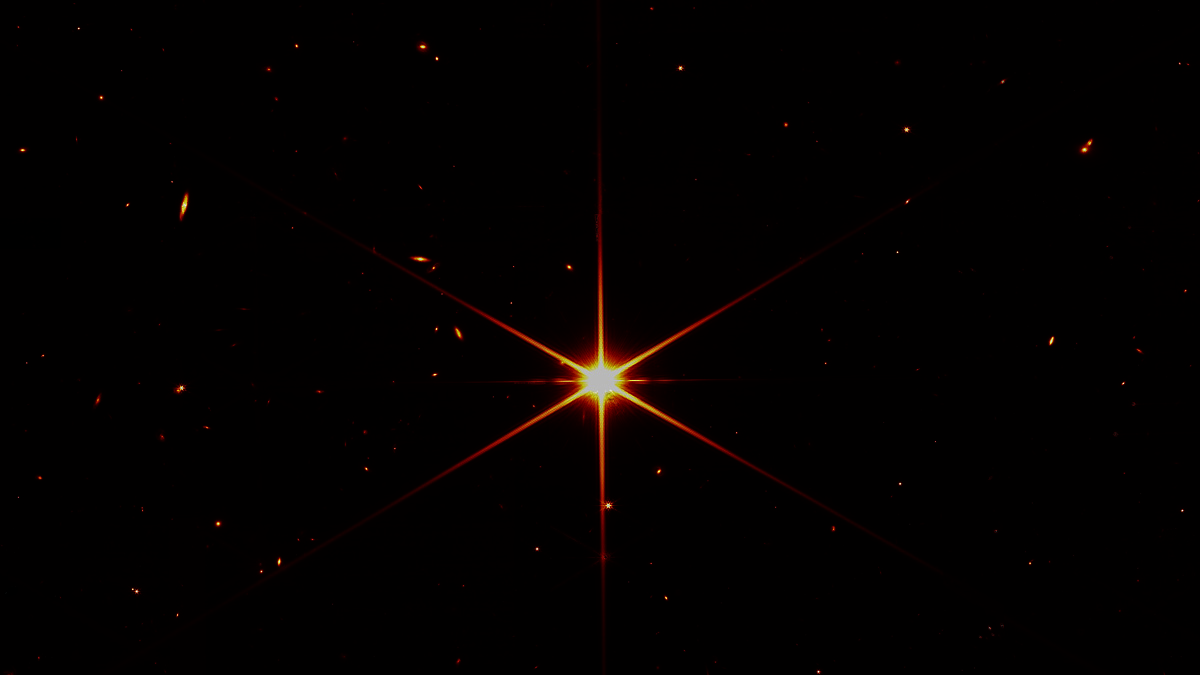
\includegraphics[width=.3\textwidth]{images/webb.png}}
    {\color{mLightBrown}\rightarrow}\
    \raisebox{-.48\height}{\includegraphics[width=.3\textwidth]{build/output/webb_mag_n.png}}
    $\cdot\exp \left(\! i\        \raisebox{-.48\height}{\includegraphics[width=.2\textwidth]{build/output/webb_phase_n.png}}\right)$

    \pause

    \centering
    \raisebox{-.48\height}{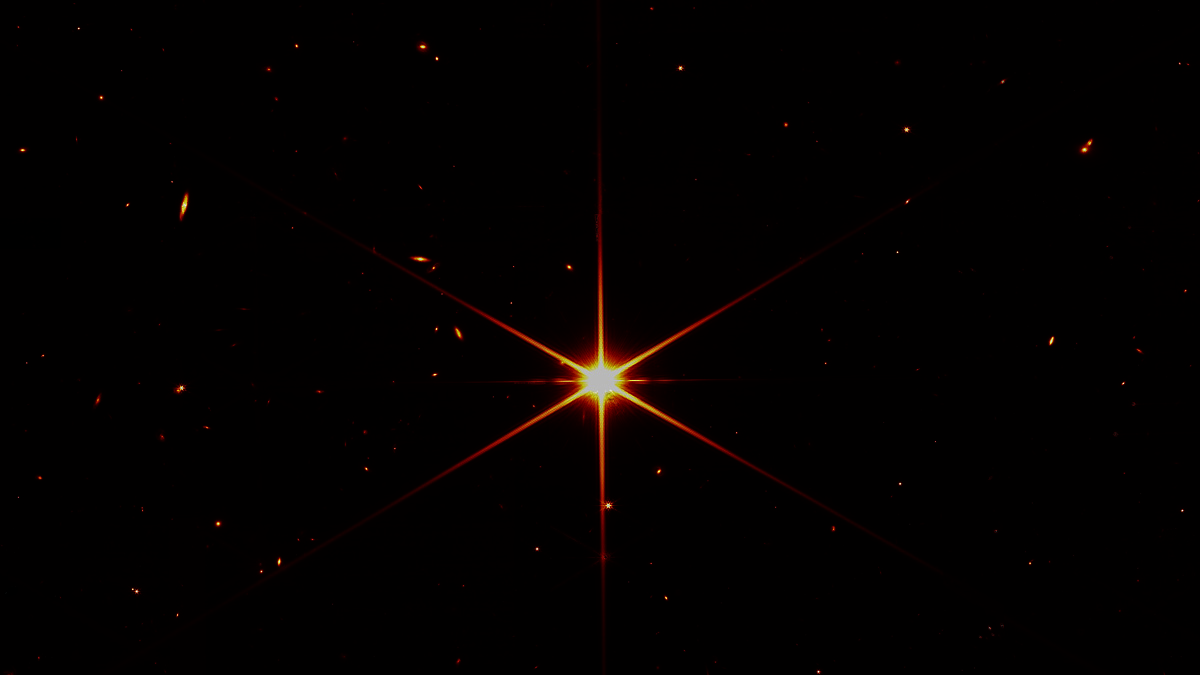
\includegraphics[width=.3\textwidth]{images/webb.png}}
    {\color{mLightBrown}\rightarrow}\
    \raisebox{-.48\height}{\includegraphics[width=.3\textwidth]{build/output/webb_mag_log.png}}
    $\cdot\exp \left(\! i\        \raisebox{-.48\height}{\includegraphics[width=.2\textwidth]{build/output/webb_phase_log.png}}\right)$

    \pause

    \centering
    \raisebox{-.48\height}{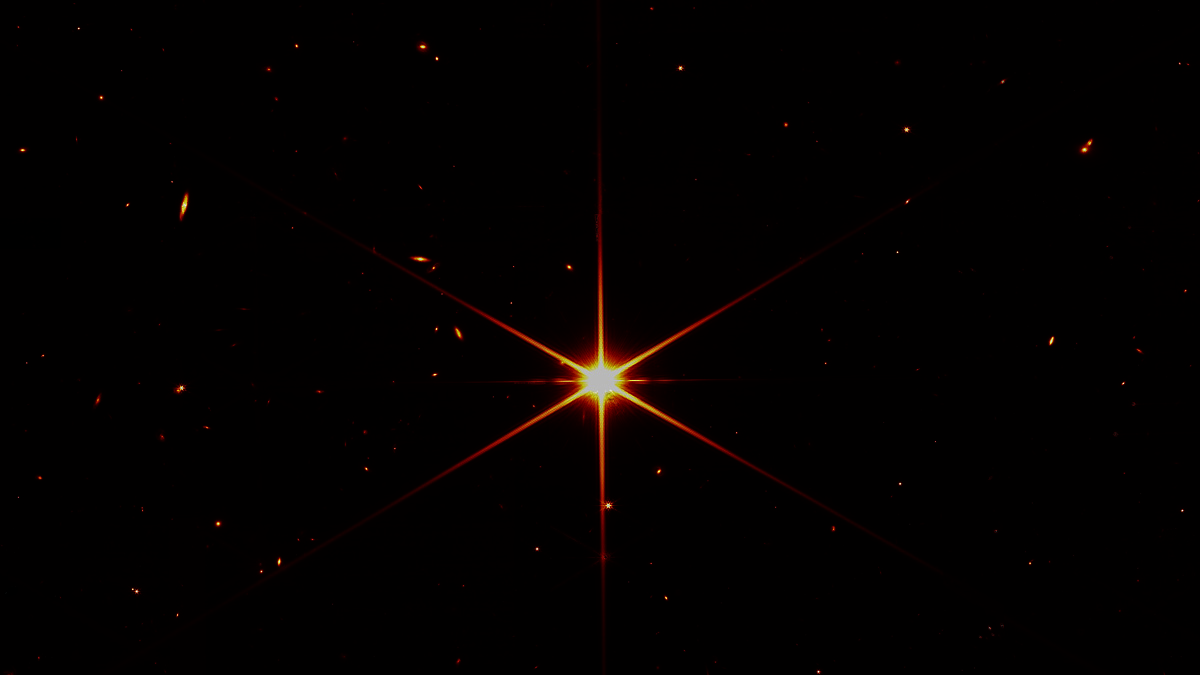
\includegraphics[width=.3\textwidth]{images/webb.png}}
    {\color{mLightBrown}\rightarrow}\
    \raisebox{-.48\height}{\includegraphics[width=.3\textwidth]{build/output/webb_mag.png}}
    $\cdot\exp \left(\! i\        \raisebox{-.48\height}{\includegraphics[width=.2\textwidth]{build/output/webb_phase.png}}\right)$
\end{frame}

\begin{frame}
    \frametitle{Editing in Fourier Space: Bluring}

    \centering
    \raisebox{-.48\height}{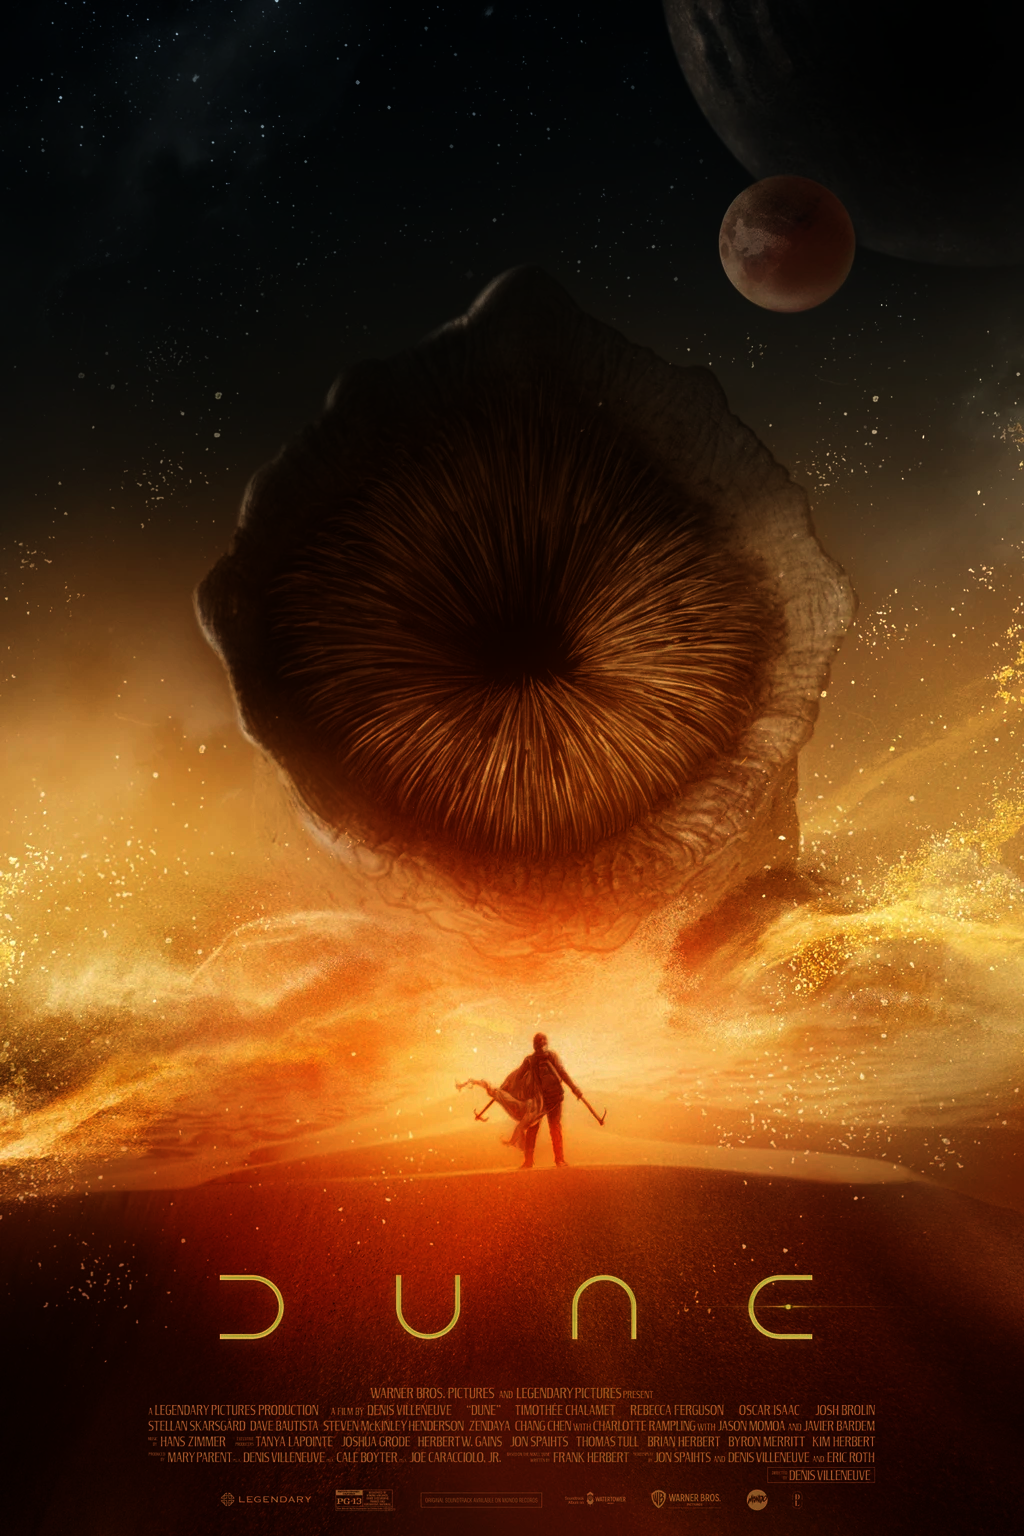
\includegraphics[width=.2\textwidth]{images/dune.png}}
    {\color{mLightBrown}\rightarrow}\
    \raisebox{-.48\height}{\includegraphics[width=.2\textwidth]{build/output/dune_mag.png}}
    {\color{mLightBrown}\rightarrow}\
    \raisebox{-.48\height}{\includegraphics[width=.2\textwidth]{build/output/dune_blur4_mask.png}}
    {\color{mLightBrown}\rightarrow}\
    \raisebox{-.48\height}{\includegraphics[width=.2\textwidth]{build/output/dune_blur4.png}}

\end{frame}

\begin{frame}
    \frametitle{Editing in Fourier Space: Bluring}

    \centering
    \raisebox{-.48\height}{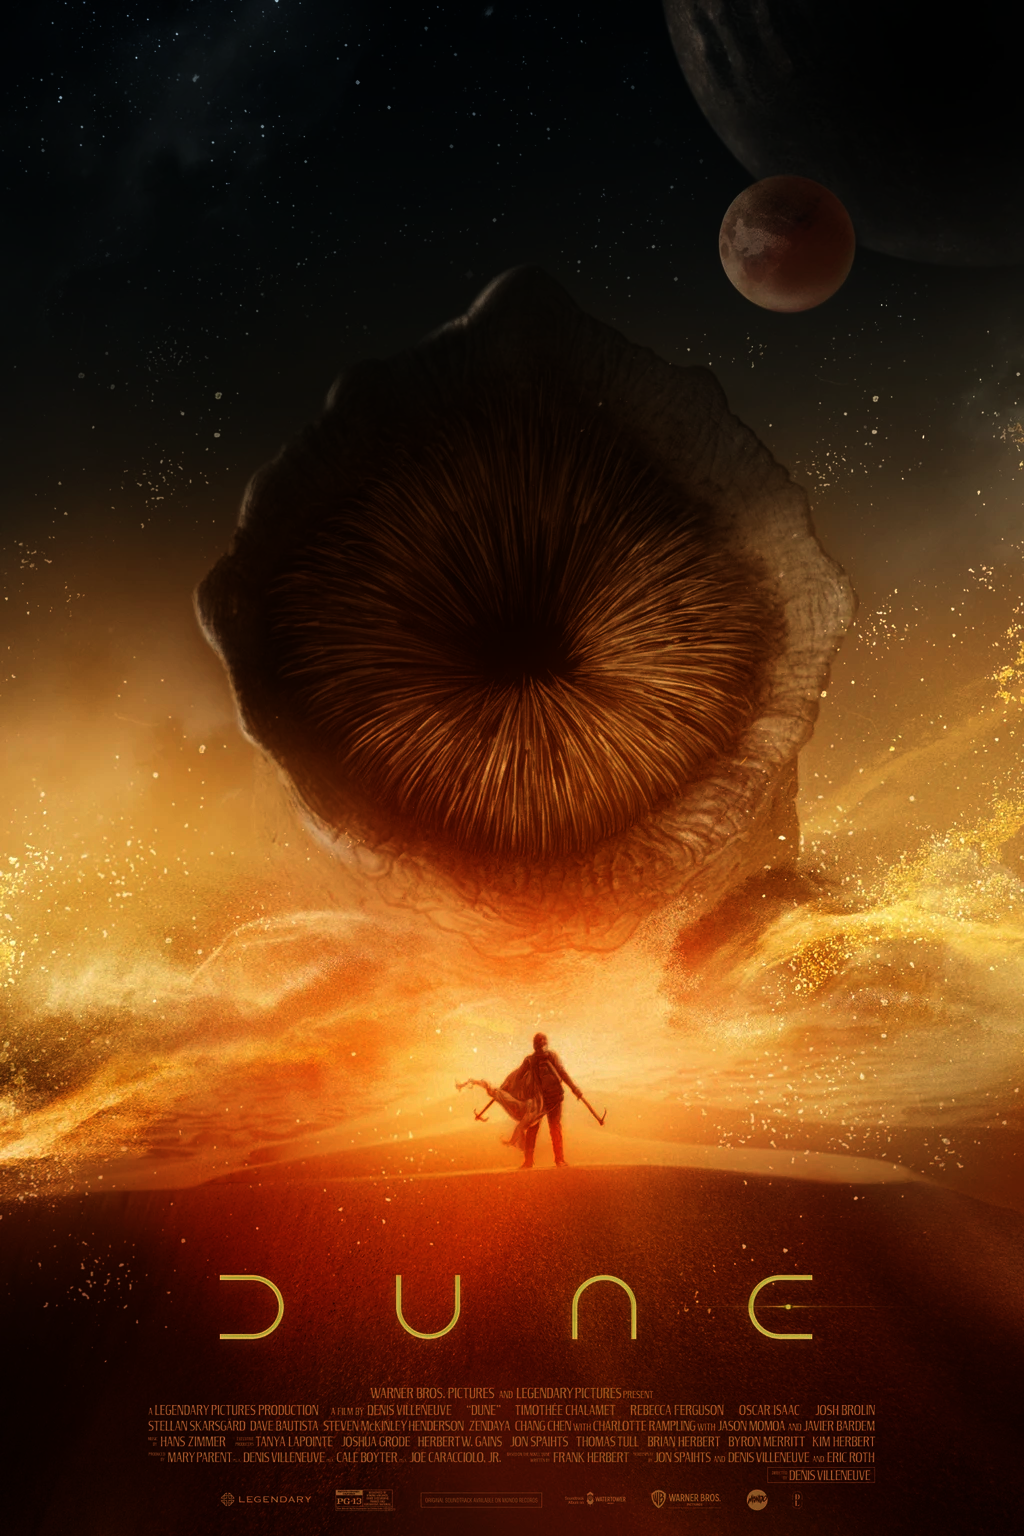
\includegraphics[width=.3\textwidth]{images/dune.png}}
    {\color{mLightBrown}\rightarrow}\
    \raisebox{-.48\height}{\includegraphics[width=.3\textwidth]{build/output/dune_blur3_mask.png}}
    {\color{mLightBrown}\rightarrow}\
    \raisebox{-.48\height}{\includegraphics[width=.3\textwidth]{build/output/dune_blur3.png}}

\end{frame}

\begin{frame}
    \frametitle{Editing in Fourier Space: Bluring}

    \centering
    \raisebox{-.48\height}{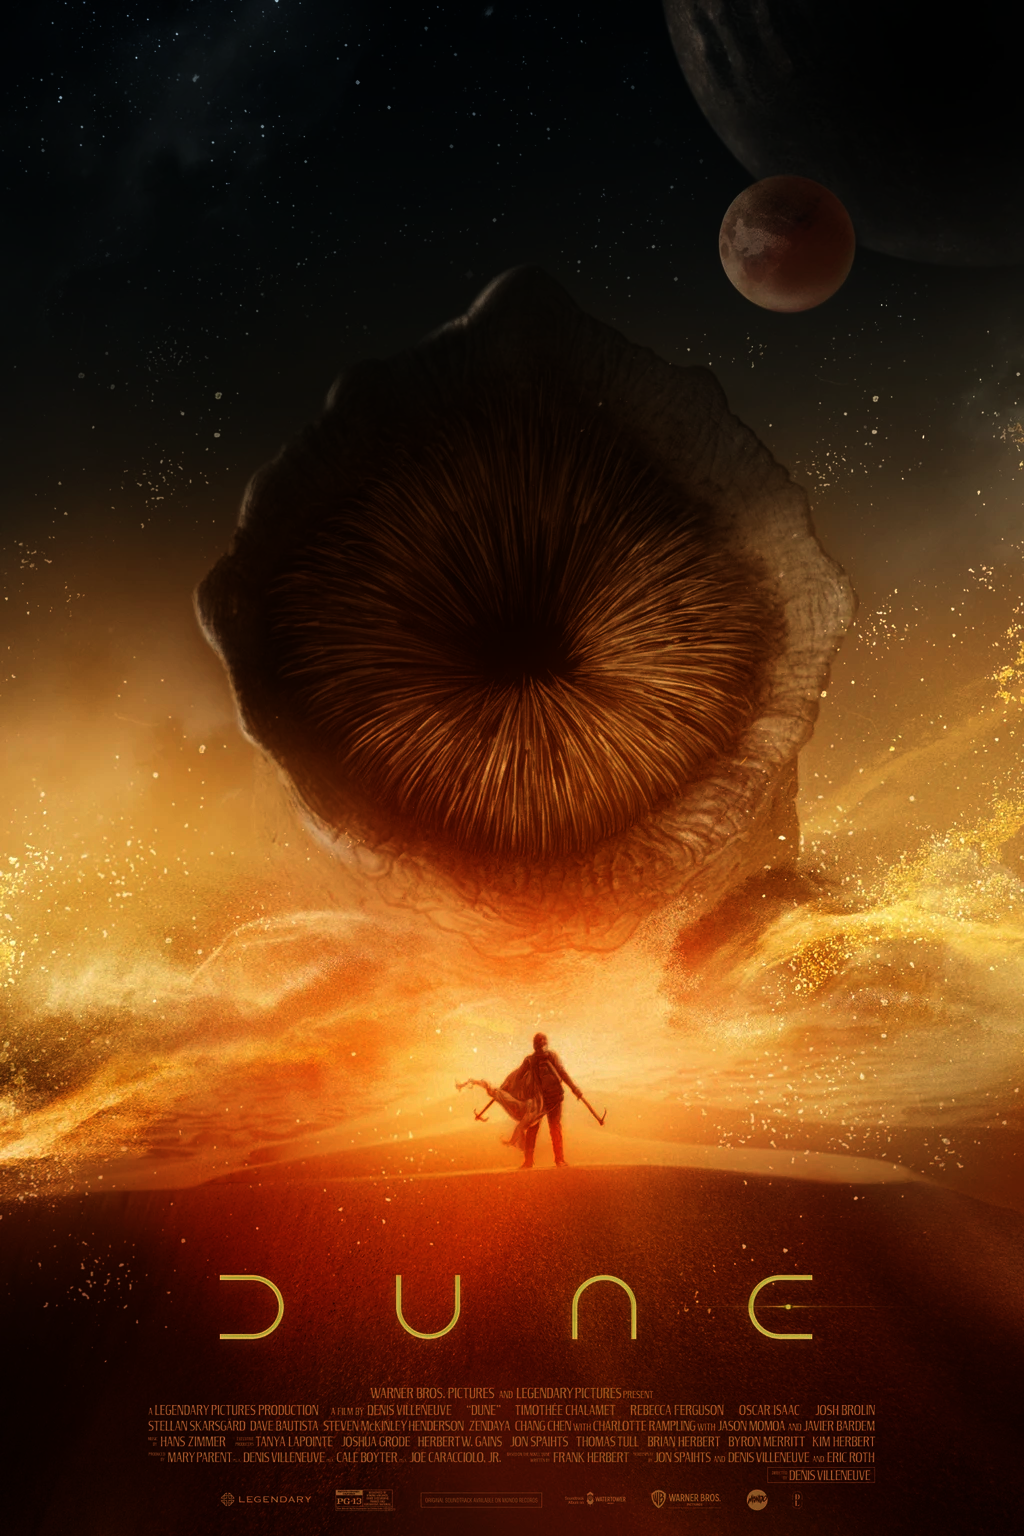
\includegraphics[width=.3\textwidth]{images/dune.png}}
    {\color{mLightBrown}\rightarrow}\
    \raisebox{-.48\height}{\includegraphics[width=.3\textwidth]{build/output/dune_blur2_mask.png}}
    {\color{mLightBrown}\rightarrow}\
    \raisebox{-.48\height}{\includegraphics[width=.3\textwidth]{build/output/dune_blur2.png}}

\end{frame}
\begin{frame}
    \frametitle{Editing in Fourier Space: Bluring}

    \centering
    \raisebox{-.48\height}{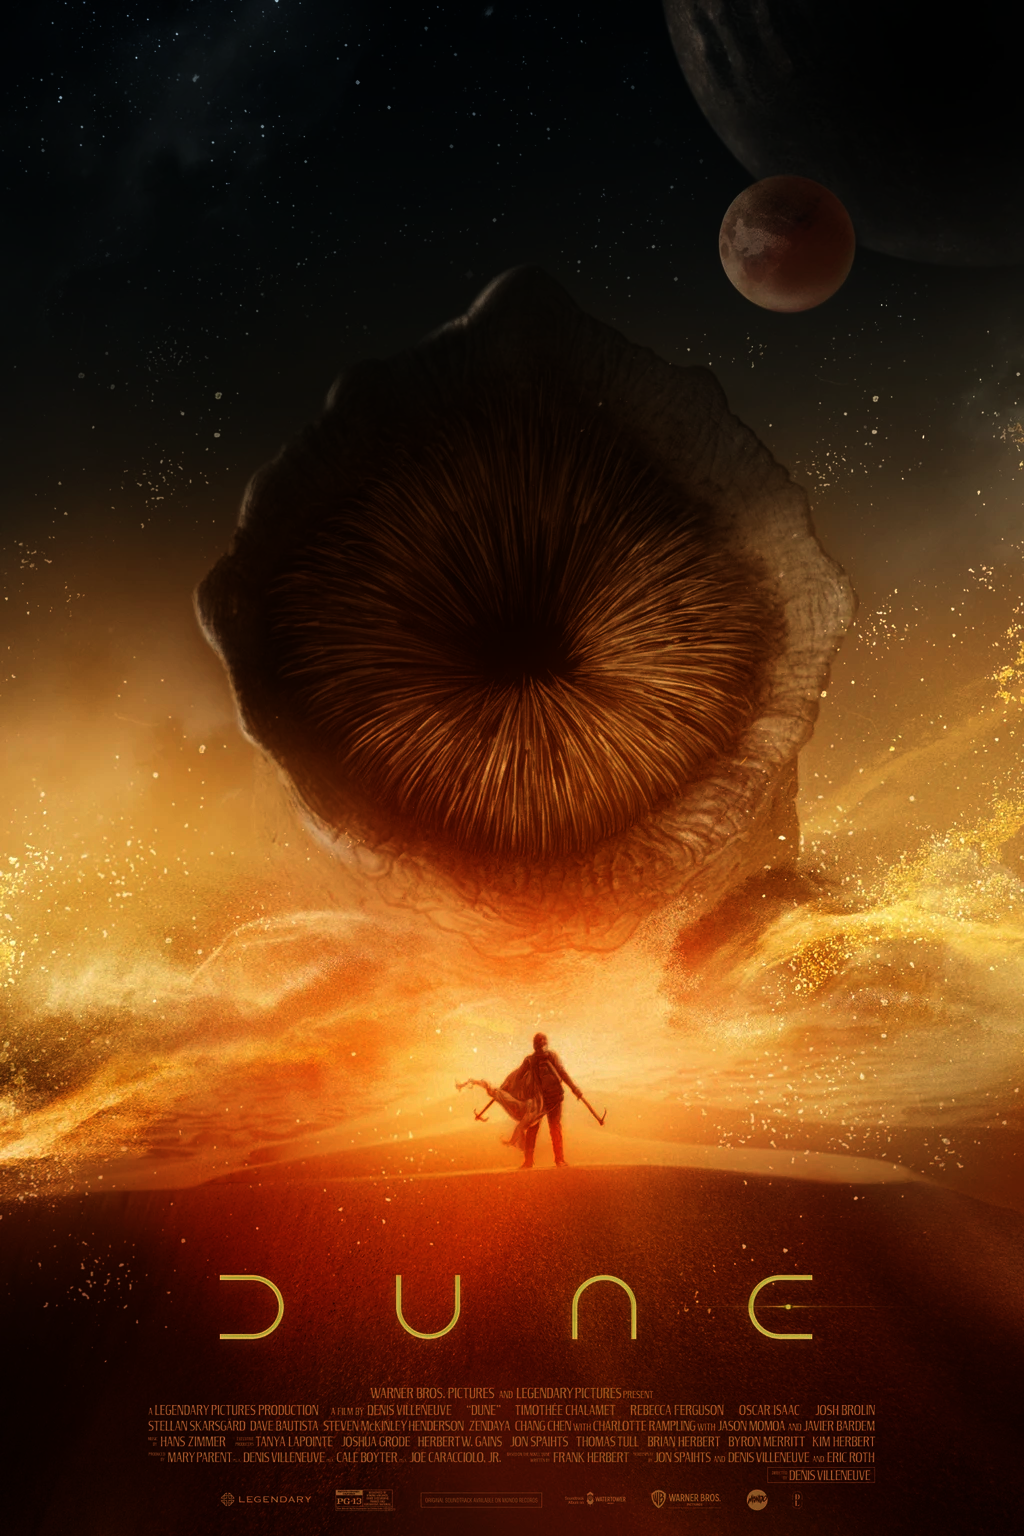
\includegraphics[width=.3\textwidth]{images/dune.png}}
    {\color{mLightBrown}\rightarrow}\
    \raisebox{-.48\height}{\includegraphics[width=.3\textwidth]{build/output/dune_blur1_mask.png}}
    {\color{mLightBrown}\rightarrow}\
    \raisebox{-.48\height}{\includegraphics[width=.3\textwidth]{build/output/dune_blur1.png}}

\end{frame}

\begin{frame}
    \frametitle{Editing in Fourier Space: Bluring}

    \centering
    \raisebox{-.48\height}{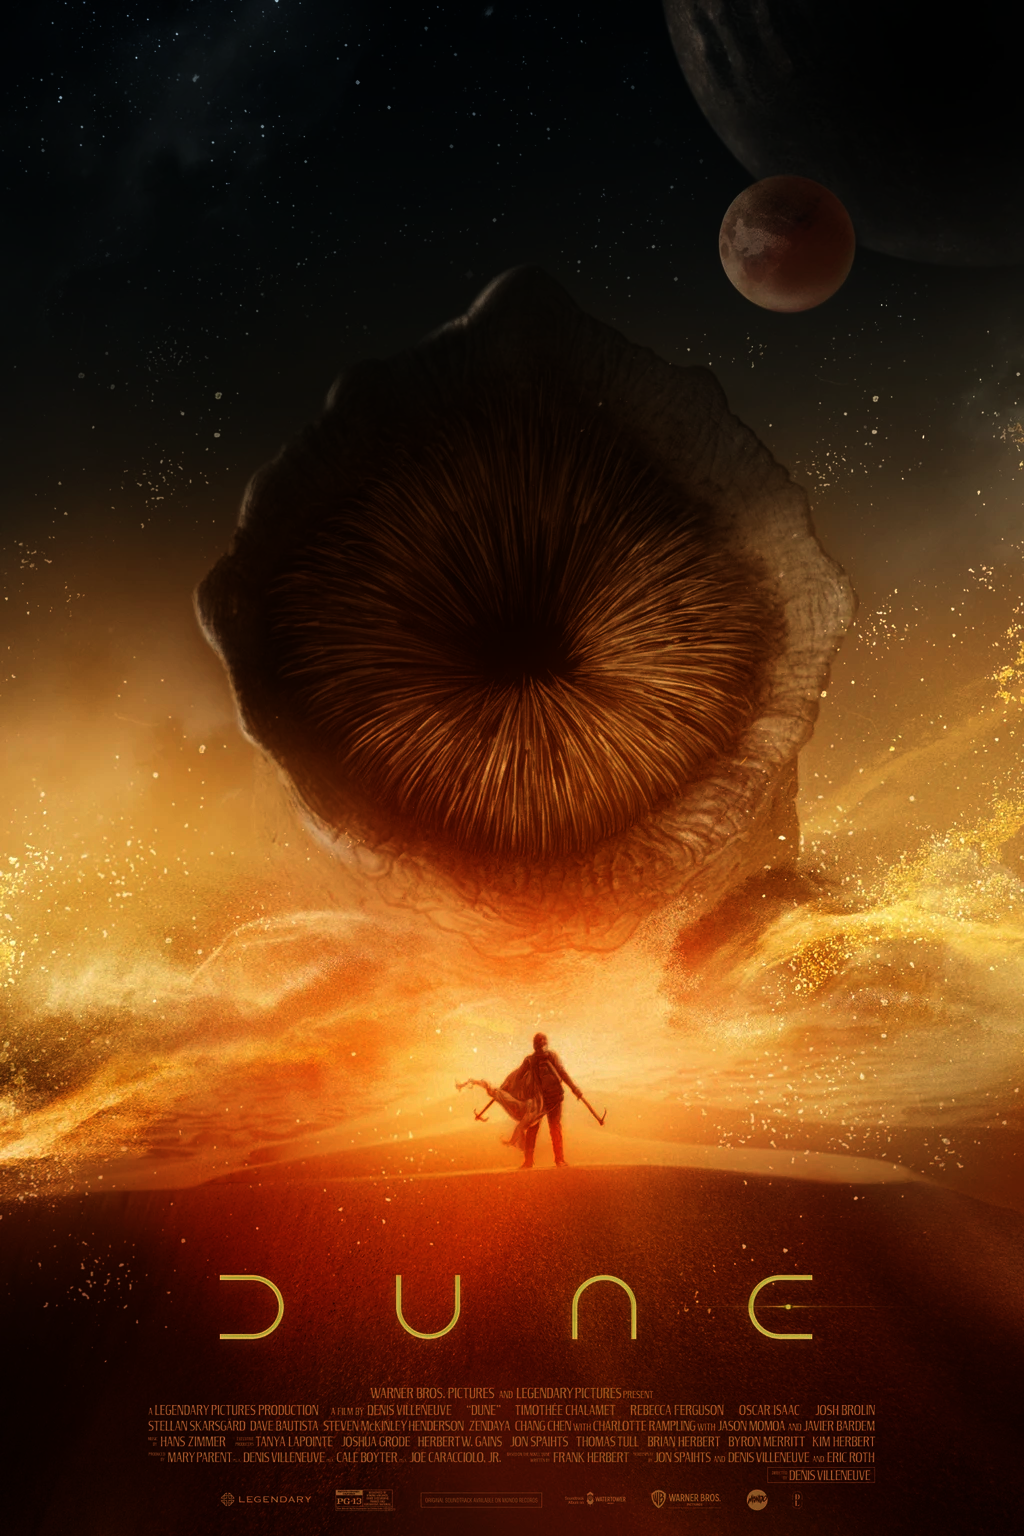
\includegraphics[width=.3\textwidth]{images/dune.png}}
    {\color{mLightBrown}\rightarrow}\
    \raisebox{-.48\height}{\includegraphics[width=.3\textwidth]{build/output/dune_blur_smooth_mask.png}}
    {\color{mLightBrown}\rightarrow}\
    \raisebox{-.48\height}{\includegraphics[width=.3\textwidth]{build/output/dune_blur_smooth.png}}

\end{frame}

\begin{frame}
    \frametitle{Editing in Fourier Space: Bluring}

    \centering
    \raisebox{-.48\height}{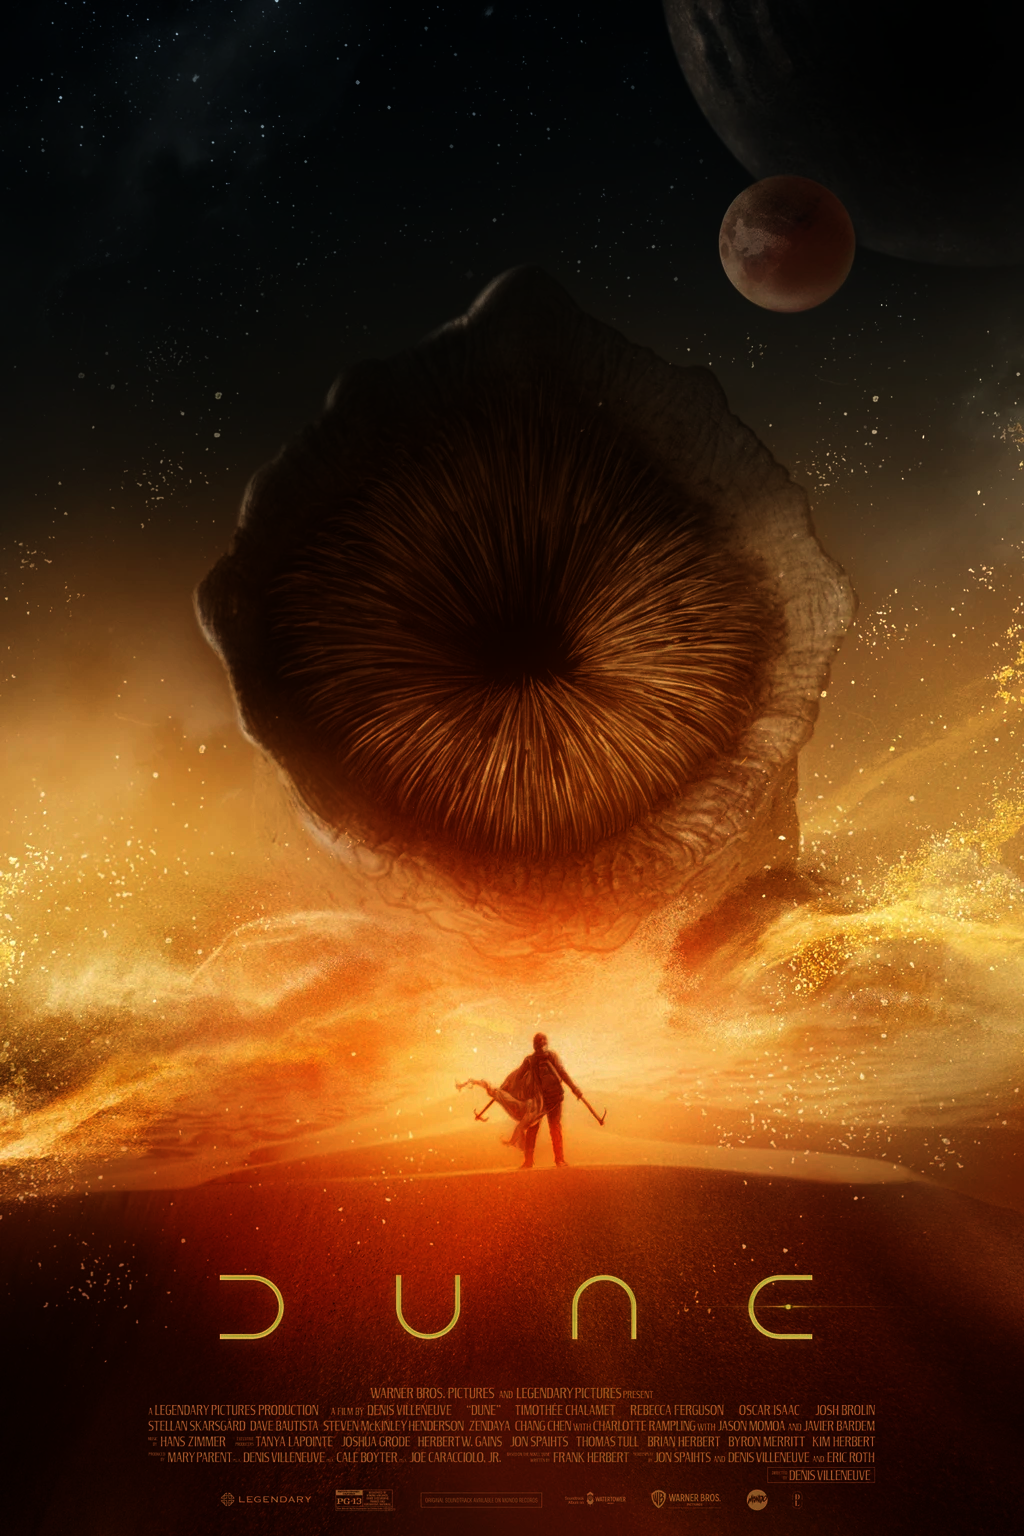
\includegraphics[width=.3\textwidth]{images/dune.png}}
    {\color{mLightBrown}\rightarrow}\
    \raisebox{-.48\height}{\includegraphics[width=.3\textwidth]{build/output/dune_rect_mask.png}}
    {\color{mLightBrown}\rightarrow}\
    \raisebox{-.48\height}{\includegraphics[width=.3\textwidth]{build/output/dune_blur_rect.png}}

\end{frame}

\begin{frame}
    \frametitle{Editing in Fourier Space: Sharpening}

    \centering
    \raisebox{-.48\height}{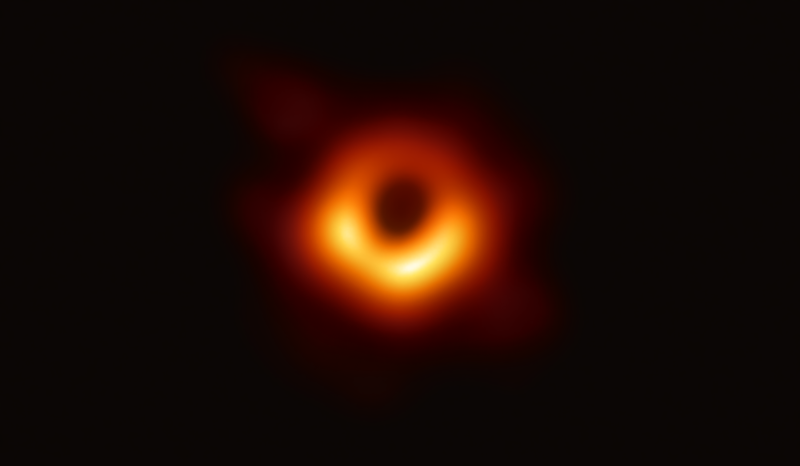
\includegraphics[width=.5\textwidth,angle=90,origin=c]{images/blackhole.png}}
    {\color{mLightBrown}\rightarrow}\
    \raisebox{-.48\height}{\includegraphics[width=.5\textwidth,angle=90,origin=c]{build/output/blackhole_sharp1_mask.png}}
    {\color{mLightBrown}\rightarrow}\
    \raisebox{-.48\height}{\includegraphics[width=.5\textwidth,angle=90,origin=c]{build/output/blackhole_sharp1.png}}

\end{frame}
\begin{frame}
    \frametitle{Editing in Fourier Space: Sharpening}

    \centering
    \raisebox{-.48\height}{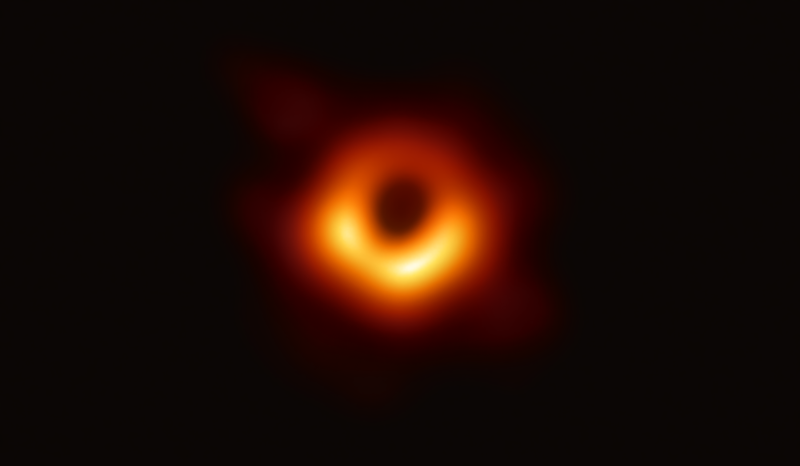
\includegraphics[width=.5\textwidth,angle=90,origin=c]{images/blackhole.png}}
    {\color{mLightBrown}\rightarrow}\
    \raisebox{-.48\height}{\includegraphics[width=.5\textwidth,angle=90,origin=c]{build/output/blackhole_sharp3_mask.png}}
    {\color{mLightBrown}\rightarrow}\
    \raisebox{-.48\height}{\includegraphics[width=.5\textwidth,angle=90,origin=c]{build/output/blackhole_sharp3.png}}

\end{frame}
\begin{frame}
    \frametitle{Editing in Fourier Space: Sharpening}

    \centering
    \raisebox{-.48\height}{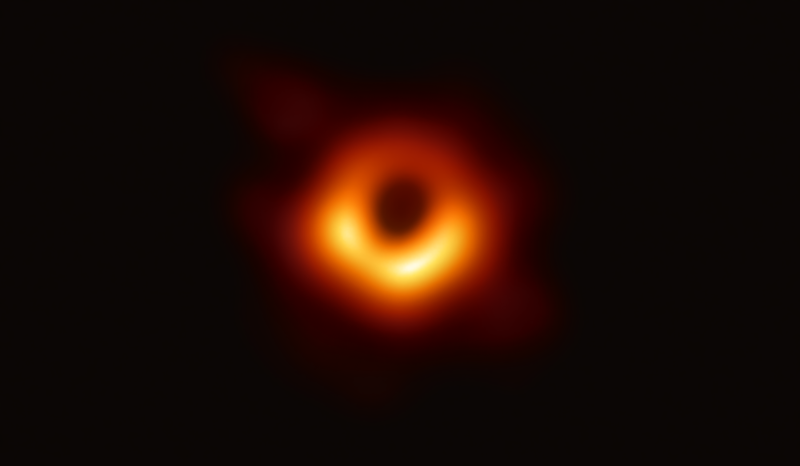
\includegraphics[width=.5\textwidth,angle=90,origin=c]{images/blackhole.png}}
    {\color{mLightBrown}\rightarrow}\
    \raisebox{-.48\height}{\includegraphics[width=.5\textwidth,angle=90,origin=c]{build/output/blackhole_sharp6_mask.png}}
    {\color{mLightBrown}\rightarrow}\
    \raisebox{-.48\height}{\includegraphics[width=.5\textwidth,angle=90,origin=c]{build/output/blackhole_sharp6.png}}

\end{frame}

\begin{frame}
    \frametitle{Editing in Fourier Space: Sharpening}

    \centering
    \raisebox{-.48\height}{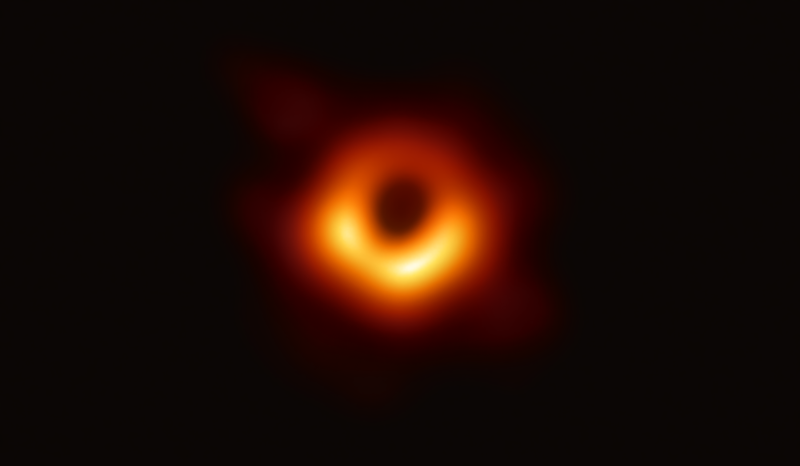
\includegraphics[width=.5\textwidth,angle=90,origin=c]{images/blackhole.png}}
    {\color{mLightBrown}\rightarrow}\
    \raisebox{-.48\height}{\includegraphics[width=.5\textwidth,angle=90,origin=c]{build/output/blackhole_sharp9_mask.png}}
    {\color{mLightBrown}\rightarrow}\
    \raisebox{-.48\height}{\includegraphics[width=.5\textwidth,angle=90,origin=c]{build/output/blackhole_sharp9.png}}

\end{frame}

\begin{frame}
    \frametitle{Editing in Fourier Space: Sharpening}

    \centering
    \raisebox{-.48\height}{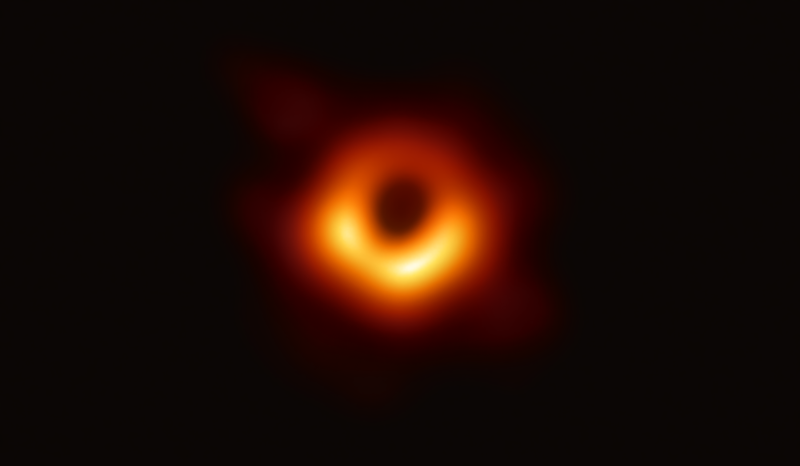
\includegraphics[width=.5\textwidth,angle=90,origin=c]{images/blackhole.png}}
    {\color{mLightBrown}\rightarrow}\
    \raisebox{-.48\height}{\includegraphics[width=.5\textwidth,angle=90,origin=c]{build/output/blackhole_sharp_smooth_mask.png}}
    {\color{mLightBrown}\rightarrow}\
    \raisebox{-.48\height}{\includegraphics[width=.5\textwidth,angle=90,origin=c]{build/output/blackhole_sharp_smooth.png}}

\end{frame}

\begin{frame}
    \frametitle{Editing in Fourier Space: Sharpening}

    \centering
    \raisebox{-.48\height}{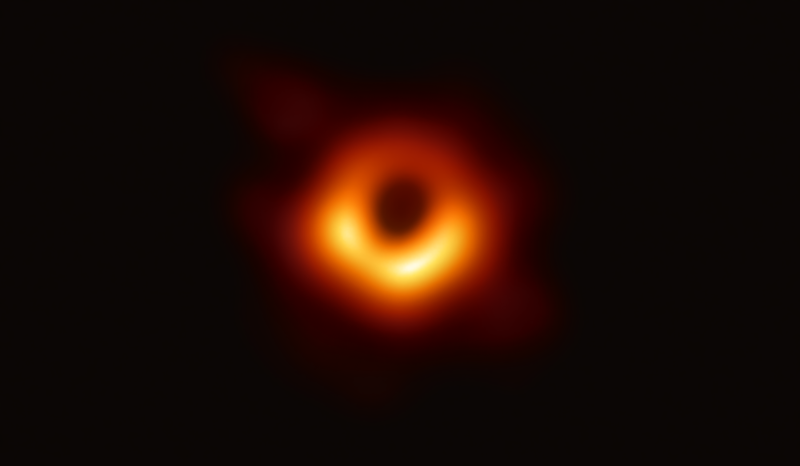
\includegraphics[width=.5\textwidth,angle=90,origin=c]{images/blackhole.png}}
    {\color{mLightBrown}\rightarrow}\
    \raisebox{-.48\height}{\includegraphics[width=.5\textwidth,angle=90,origin=c]{build/output/blackhole_sharp_smooth_mask_g.png}}
    {\color{mLightBrown}\rightarrow}\
    \raisebox{-.48\height}{\includegraphics[width=.5\textwidth,angle=90,origin=c]{build/output/blackhole_sharp_smooth_g.png}}

\end{frame}

\begin{frame}{Diffraction}
    In the Fraunhofer-Approximation the diffraction image is the FT of the aperture
    \begin{equation*}
        A(x, y, z) \propto \iint_{\symup{Aperture}}\hspace{-3em} e^{-i\frac{2\pi}{\lambda z}(x'x+y'y)} \dif x' \dif y'
    \end{equation*}
    Now we can numerically simulate this

    \centering
    \raisebox{-.48\height}{
\includegraphics[width=.3\textwidth]{images/double_slit_small_norm.png}}
    {\color{mLightBrown}\rightarrow}\
    \raisebox{-.48\height}{\includegraphics[width=.3\textwidth]{build/output/double_slit_small_norm_mag.png}}

\end{frame}
\begin{frame}{Diffraction}
    \centering
    \raisebox{-.48\height}{\includegraphics[width=.25\textwidth]{images/double_slit_small_norm.png}}
    {\color{mLightBrown}\rightarrow}\
    \raisebox{-.48\height}{\includegraphics[width=.25\textwidth]{build/output/double_slit_small_norm_mag.png}}

    \raisebox{-.48\height}{\includegraphics[width=.25\textwidth]{images/double_slit_small_close.png}}
    {\color{mLightBrown}\rightarrow}\
    \raisebox{-.48\height}{\includegraphics[width=.25\textwidth]{build/output/double_slit_small_close_mag.png}}
\end{frame}

\begin{frame}{Diffraction}
    \centering
    \raisebox{-.48\height}{\includegraphics[width=.25\textwidth]{images/double_slit_small_widest.png}}
    {\color{mLightBrown}\rightarrow}\
    \raisebox{-.48\height}{\includegraphics[width=.25\textwidth]{build/output/double_slit_small_widest_mag.png}}

    \raisebox{-.48\height}{\includegraphics[width=.25\textwidth]{images/double_slit_norm_widest.png}}
    {\color{mLightBrown}\rightarrow}\
    \raisebox{-.48\height}{\includegraphics[width=.25\textwidth]{build/output/double_slit_norm_widest_mag.png}}
\end{frame}

\begin{frame}{Diffraction}
    \centering
    \raisebox{-.48\height}{\includegraphics[width=.25\textwidth]{images/hole.png}}
    {\color{mLightBrown}\rightarrow}\
    \raisebox{-.48\height}{\includegraphics[width=.25\textwidth]{build/output/hole_mag.png}}

    \raisebox{-.48\height}{\includegraphics[width=.25\textwidth]{images/hole_tiny.png}}
    {\color{mLightBrown}\rightarrow}\
    \raisebox{-.48\height}{\includegraphics[width=.25\textwidth]{build/output/hole_tiny_mag.png}}
\end{frame}
\begin{frame}{Compression}
    \begin{itemize}
        \item The eye is not sensitive to small differences in Fourier-space
        \item[$\rightarrow$] Only save a sub-set of Fourier-coefficients, to lossy-compress the image
        \item This is what \texttt{.jpg} does
        \item Only Problem: Complex numbers
    \end{itemize}

\end{frame}
\begin{frame}{DCT}
    Let's stay real!
    \begin{align*}
        X_k =\frac{2c_k}{\sqrt N}\sum_{n=0}^{N-1}x_n \cos \left(\frac{\pi\left(2n+1\right)k}{2N} \right)
        \qquad \leftrightarrow & \qquad
        x_k
        =\frac{1}{\sqrt N}\sum_{n=1}^{N-1}c_n X_n \cos \left(\frac{\pi(2k+1)}{2N}n\right)
        \\
        \text{where }
        c_k =                  &
        \begin{cases}
            \frac{1}{\sqrt{2}} \quad & k=0           \\
            1                        & \text{ else }
        \end{cases}
    \end{align*}
    An efficient algorithm based on FFT\footnote{\fullcite{DCTUFFT}}:
    \begin{align*}
        \begin{rcases}
            x'_k       & = x_{2k}  \\
            x'_{N-1-k} & =x_{2k+1}
        \end{rcases}
        k=0,1, \dots, \frac{N}{2}-1
        \quad & \Rightarrow
        X_k =2 c_k
        \Re e^{i\pi\frac{k}{2N}}\symcal{F}^{-1}\left(\vec x'\right)_k
        \\
        x_{2k} =
        \Re \symcal{F}^{-1}\left\{c_lX_le^{i\frac{\pi l}{2N}}\right\}_k
        \qquad
              & x_{2k+1} = x_{2(N-1-k)}
    \end{align*}
\end{frame}

\begin{frame}
    \frametitle{Naive Compression: Low Coefficient Cutoff}
    \centering

    \raisebox{-.48\height}{\includegraphics[width=.2\textwidth]{images/A.png}}

    {\color{mLightBrown}\downarrow}\

    \begin{tabular}{c c c c}
        \includegraphics[width=.2\textwidth]{build/plots/A9.png}
         & \includegraphics[width=.2\textwidth]{build/plots/A5.png}
         & \includegraphics[width=.2\textwidth]{build/plots/A2.png}
         & \includegraphics[width=.2\textwidth]{build/plots/A1.png}
        \\10\% & 50\%                                                     & 80\% & 90\%
    \end{tabular}

\end{frame}

\begin{frame}
    \frametitle{Naive Compression: Low Coefficient Cutoff}
    Was I actually able to reduce the size of the new file-format? \rightarrow No
    \begin{itemize}
        \item We must additionally save the index
        \item The coefficients must be saved as float (compared to the uint8 pixel type)
        \item .jpg does not DCT the whole image, but $8\times 8$ sub-images
        \item .jpg quantizes DCT-coefficients (lossy), so that non-lossy compression algorithms work at full-power
    \end{itemize}

\end{frame}